\documentclass{article}

\usepackage{polski}
\usepackage{amsmath}
\usepackage{graphicx}
\usepackage{float}
\usepackage{xcolor}

\newsavebox\MBox
\newcommand\Cline[2][red]{{\sbox\MBox{$#2$}%
  \rlap{\usebox\MBox}\color{#1}\rule[-1.2\dp\MBox]{\wd\MBox}{0.5pt}}}

\title{Sprawozdanie 1: Bramki i funkcje logiczne}
\author{\textbf{Jakub Szymczak, Damian Tworek,}\\ \textbf{Maksymilian Sulima, Łukasz Wala} \\
    \textit{AGH, Wydział Informatyki, Elektroniki i Telekomunikacji} \\
    \textit{Technika Cyfrowa 2021/2022}}
\date{Kraków, \today}

\begin{document}
\maketitle



\section{Ćwiczenie \textit{1a}}
Ideą ćwiczenia jest zaprojetowanie, zbudowanie i przetestowanie układu realizującego funkcję logiczną:
\[\mathbf{Y=\overline{A}C+B(A+B)}\]

\begin{figure}[H]
    \centering
    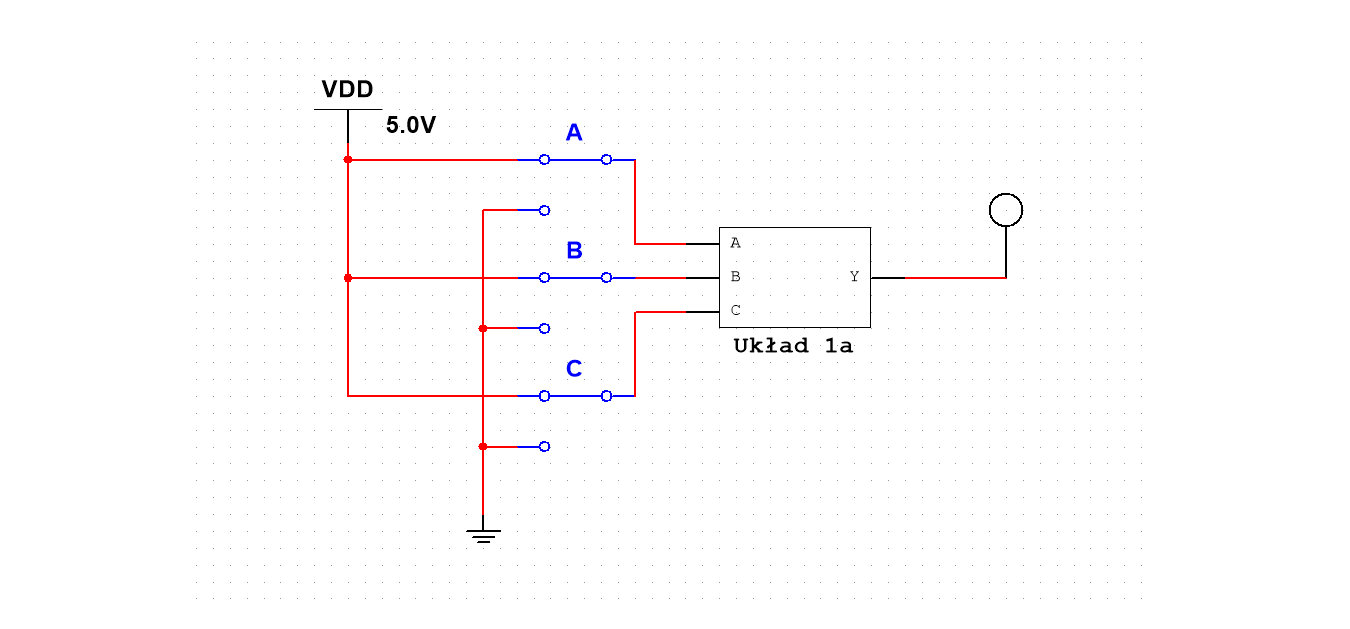
\includegraphics[width=\textwidth]{idea_1.png}
    \caption{Układ 1a}
\end{figure}

\subsection{Rozwiązanie teoretyczne}
Rozpocznijmy od przekształcenia funkcji logicznej do postaci zawierającej tylko koniunkcje i zaprzeczenia. 
Korzystając z prawa rozdzielności koniunkcji względem alternatywy
\[\mathbf{Y=\overline{A}C+BA+BB}\]
Tutaj można zauważyć, że $\mathbf{BB=B}$, więcej
\[\mathbf{Y=\overline{A}C+BA+B}\]
Ponownie korzystając z prawa rozdzielności koniunkcji względem alternatywy
\[\mathbf{Y=\overline{A}C+B(A+1)}\]
Tutaj $\mathbf{A+1=1}$, więc
\[\mathbf{Y=\overline{A}C+B}\]
Używając prawa de Morgana
\[\mathbf{Y=\overline{\overline{\overline{A}C}\overline{B}}}\]

\subsection{Implementacja w programie Multisim}
Do zbudowania układu wykorzystano 4 bramki NAND, diodę LED, generator słów oraz analizator logiczny.
Przedstawiony jest na \textbf{rysunku 2}.
Na podstawie prawa de Morgana oraz prawa rozdzielności alternatywy względem koniunkcji
\[\mathbf{\overline{AA}=\overline{A}+\overline{A}=\overline{A}(1+1)=\overline{A}}\]
więc bramka NAND może posłużyć jako NOT, jeżeli do obu wejść podany zostanie ten sam sygnał.
\[\mathbf{Y=\overline{\overline{\overline{A}^1C}^3\overline{B}^2}}^4\]


\begin{figure}[H]
    \centering
    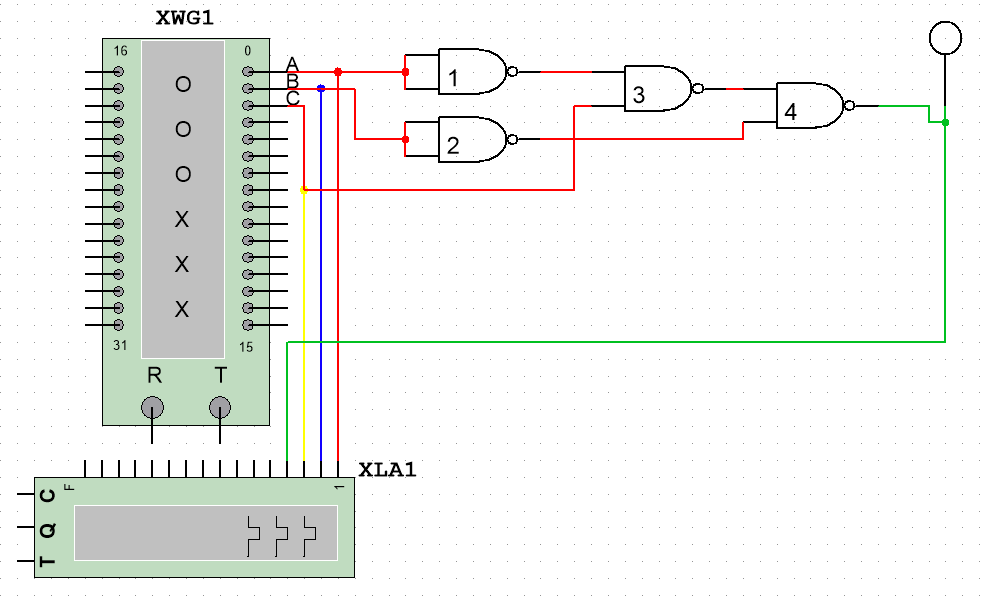
\includegraphics[width=\textwidth]{uklad_1.png}
    \caption{Układ logiczny w programie Multisim na podstawie przekształconej funkcji}
\end{figure}

\begin{figure}[H]
    \centering
    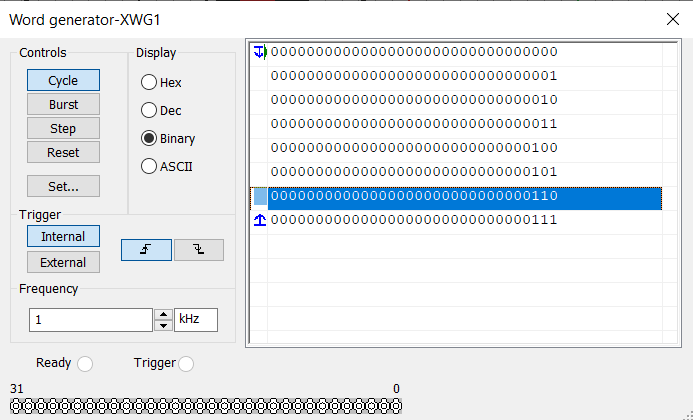
\includegraphics[width=\textwidth]{generator_1.png}
    \caption{Generator słów dla pierwszego układu}
\end{figure}

Za pomocą analizatora logicznego zbadane zostały przebiegi czasowe badanego układu przedstawione na 
\textbf{rysunku 4} (\textbf{A} - czerwony, \textbf{B} - niebieski, \textbf{C} - żólty, \textbf{Y} - zielony).

\begin{figure}[H]
    \centering
    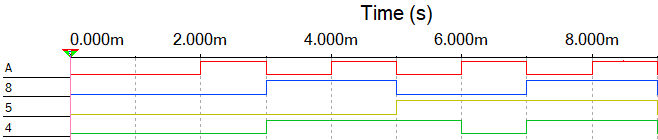
\includegraphics[width=\textwidth]{analiza_1.png}
    \caption{Wykres przebiegu czasowego badanego układu}
\end{figure}

Ponizej na \textbf{rysunkach 5 i 6} automatycznie wygenerowany układ na podstawie funkcji przed przekształceniami, wyniki są zgodne dla obu wariantów,
co potwierdza poprawność funkcji po przekształceniu.

\begin{figure}[H]
    \centering
    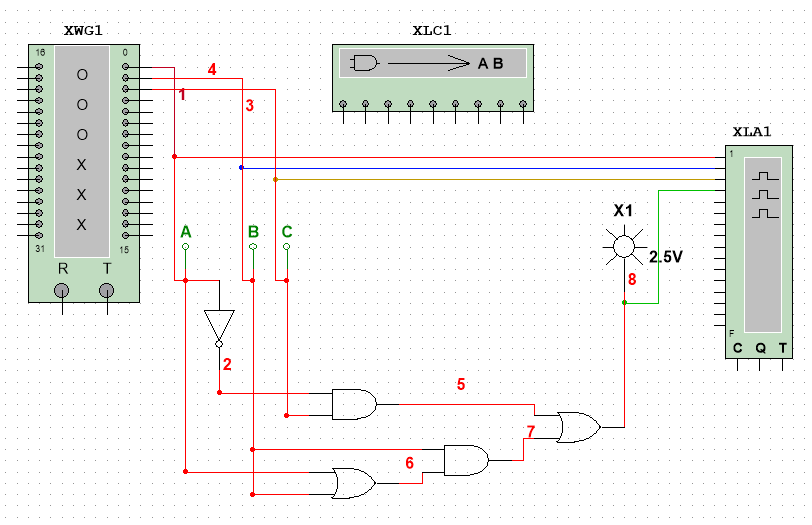
\includegraphics[width=\textwidth]{uklad_1_wyg.png}
    \caption{Układ logiczny wygenerowany przez Multisim na podstawie funkcji przed przekształceniami}
\end{figure}

\begin{figure}[H]
    \centering
    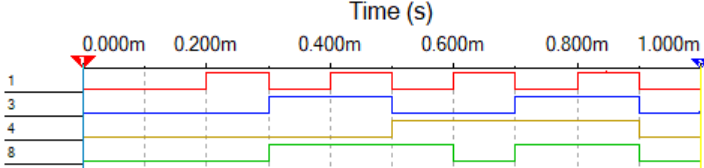
\includegraphics[width=\textwidth]{analiza_1_wyg.png}
    \caption{Wykres przebiegu czasowego badanego układu (przed przekształceniami)}
\end{figure}

Poniżej (\textbf{na rysunku 7}) znajduję się automatyczny układ testujący sprawdzający poprawność działania układu

\begin{figure}[H]
    \centering
    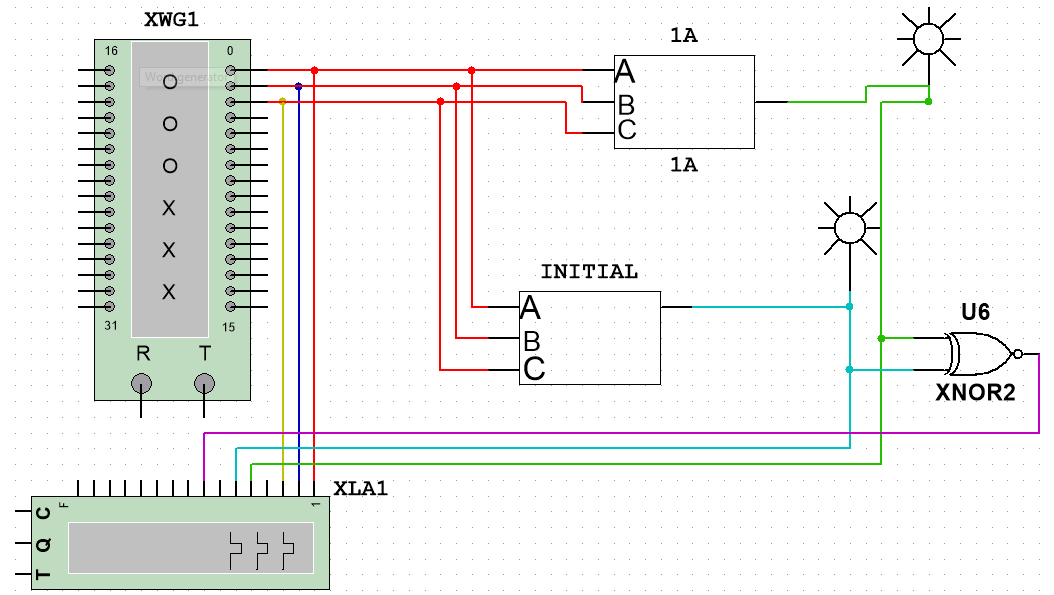
\includegraphics[width=\textwidth]{test_1.png}
    \caption{Automatyczny układ testujący dla układu 1a}
\end{figure}

\begin{figure}[H]
    \centering
    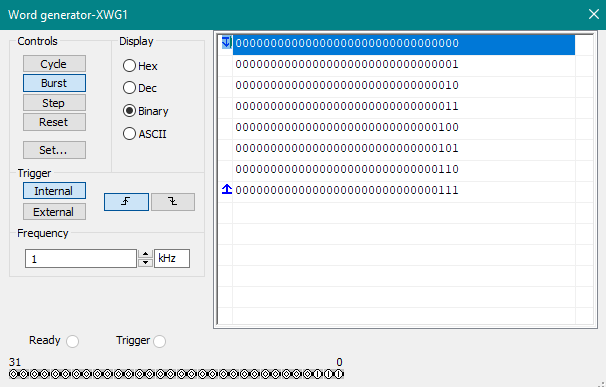
\includegraphics[width=\textwidth]{generator_test_1.png}
    \caption{Generator słów dla układu testującego}
\end{figure}

\begin{figure}[H]
    \centering
    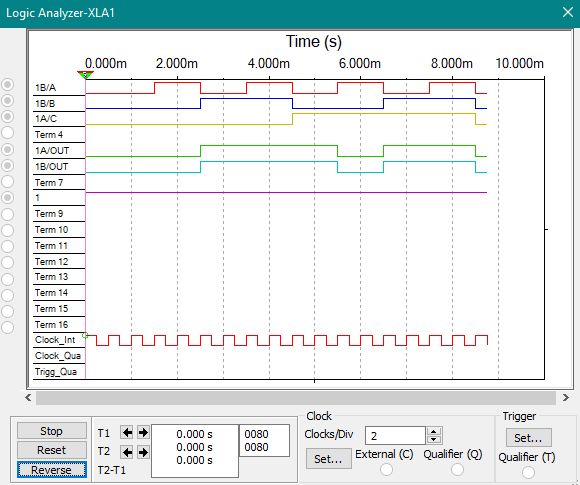
\includegraphics[width=\textwidth]{analiza_test_1.png}
    \caption{Analiza dla układu testującego}
\end{figure}

\subsection{Wnioski}

\begin{itemize}
    \item
    W rzeczywistości ceny i dostępność różnych bramek różnią się, dlatego w tym przypadku opłacalna była zmiana na bramki NAND 
    ze względu na ich niską cenę.
    \item
    Przekształcając funkcję zgodnie z prawami logiki zmniejszyliśmy liczbę elementów potrzebnych do stworzenia układu 
    (z 3 elementów (bramki OR, AND, OR) do jednego elementu z 4 bramkami NAND).
    \item
    Układ może być zastosowany jako asynchroniczny przerzutnik "RS". Jeżeli podstawimy:
    \[S:=B, \quad R:=A, \quad Q_{n-1}:=C, \quad Q_n=Y\]
    Wówczas otrzymujemy funkcję charakteryzującą stan kolejny stan przerzutnika.
    \[Q_n=S+\overline{R}Q_{n-1}\]
    
\end{itemize}



\section{Ćwiczenie \textit{1b}}
Ideą ćwiczenia jest zaprojektowanie, zbudowanie i przetestowanie układu, który sprawdza, czy liczba w postaci czterobitowego słowa jest pierwsza. 

\begin{figure}[H]
    \centering
    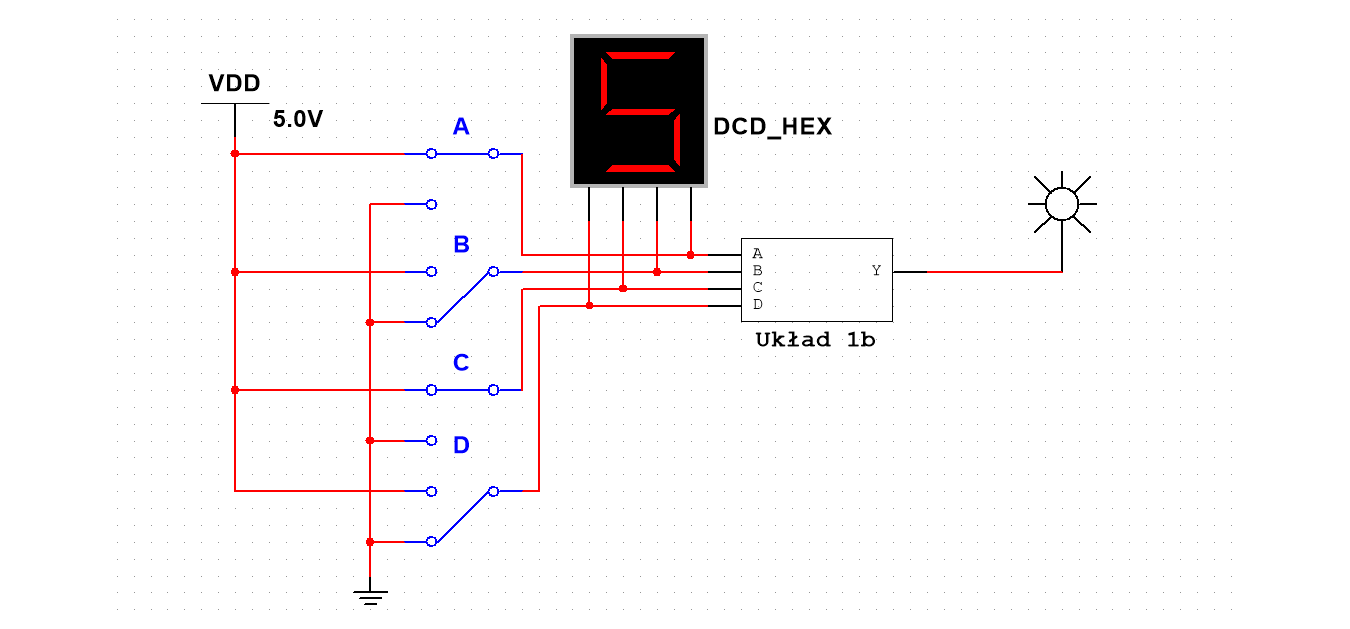
\includegraphics[width=\textwidth]{idea_2.png}
    \caption{Układ 1b}
\end{figure}

\subsection{Rozwiązanie teoretyczne}
Do zaprojektowania układu użyta została funkcja
    \[f(A,B,C,D)=\sum{m_i}, i\in\{2,3,5,7,11,13\}\]
Gdzie $m_i$ odpowiada iloczynowi logicznemu każdego z argumentów funkcji lub jego zaprzeczenia 
odpowiadającemu zapisowi na czterech bitach liczby $i$.
Do jej uproszczenia posłuży tablica Karnough przedstawiona na \textbf{rysunku 11}.

\begin{figure}[H]
    \centering
    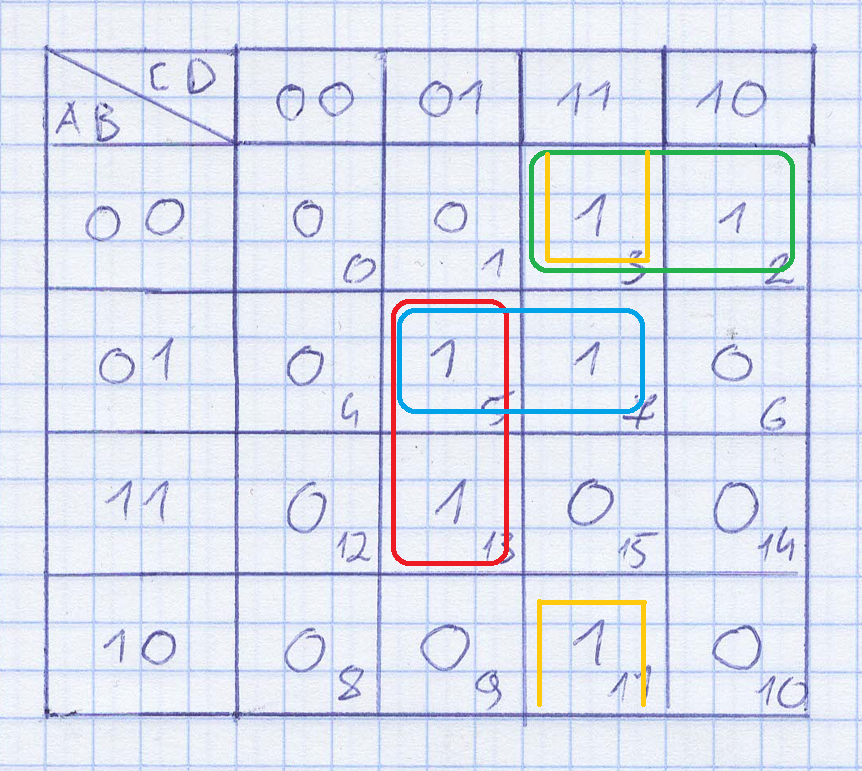
\includegraphics[width=\textwidth]{tabela_1.png}
    \caption{Tabela Karnough dla jedynek}
\end{figure}

Funkcja po uproszczeniu wygląda następująco
\[f(A,B,C,D)=\Cline[blue]{\overline{A}BD}+\Cline[green]{\overline{A}\:\overline{B}C}+\Cline[red]{B\overline{C}D}+\Cline[yellow]{\overline{B}CD}\]

Korzystając z rozdzielności koniunkcji względem alternatywy
\[f(A,B,C,D)=\overline{B}C(\overline{A}+D)+BD(\overline{A}+\overline{C})\]

Poniżej tablica Karnough z wykorzystanie zaznaczania zer (\textbf{rysunek 12}).
\begin{figure}[H]
    \centering
    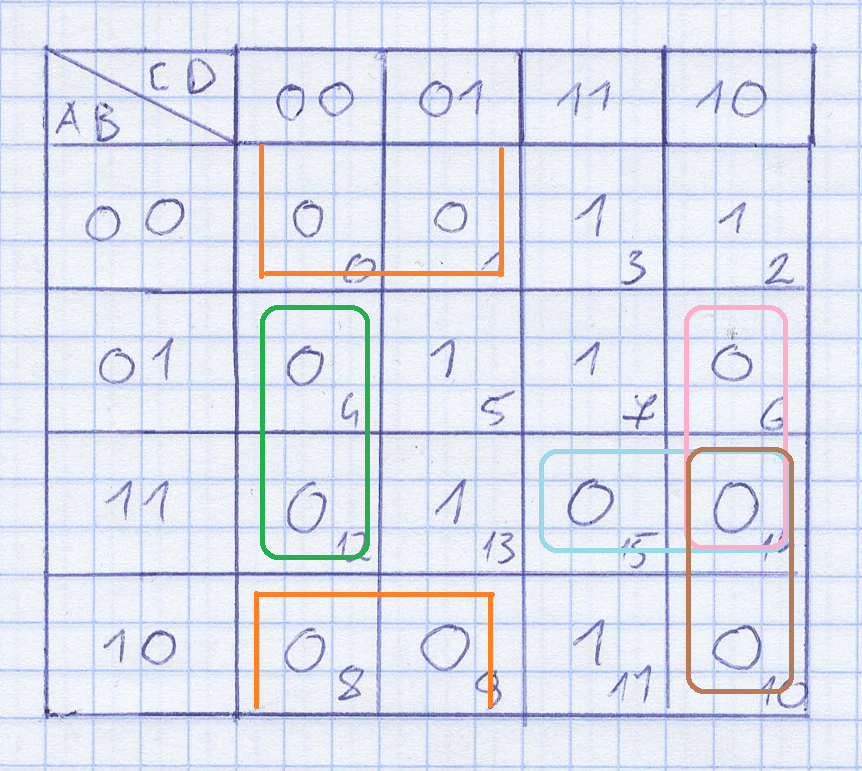
\includegraphics[width=\textwidth]{tabela_0.png}
    \caption{Tabela Karnough dla zer}
\end{figure}

Po uproszczeniu na podstawie tablicy Karnough z wykorzystaniem zer funkcja wygląda następująco
\[f(A,B,C,D)=\Cline[orange]{(C+B)}\Cline[pink]{(\overline{C}+D+\overline{B})}\Cline[cyan]{(\overline{A}+\overline{B}+\overline{C})}\Cline[brown]{(\overline{C}+D+\overline{A})}\Cline[green]{(C+D+\overline{B})}\]
Ze względu na jej większy poziom skomplikowania wybraliśmy funkcję przekształconą na podstawie tablicy z wykorzystanie zaznaczania jedynek.


\subsection{Implementacja w programie Multisim}
Układ (\textbf{na rysunku 13}) skonstruowany został na podstawie równania przekształconego z użyciem tablicy Karnough dla jedynek. 
Alternatywny, bazowany
na tym samym równaniu, ale po zastosowaniu zasady rozdzielności koniunkcji względem alternatywy, 
używa tyle samo, ale innych rodzajów bramek (3 bramek NOT, 3 bramek OR dwuargumentowych, 
2 bramek AND trzyargumentowych). Poniżej znadjują się obie wersje układu, odczyty generatora słów dotyczą obu układów.

\[Y=\overline{A}BD+\overline{A}\:\overline{B}C+B\overline{C}D+\overline{B}CD\]
\begin{figure}[H]
    \centering
    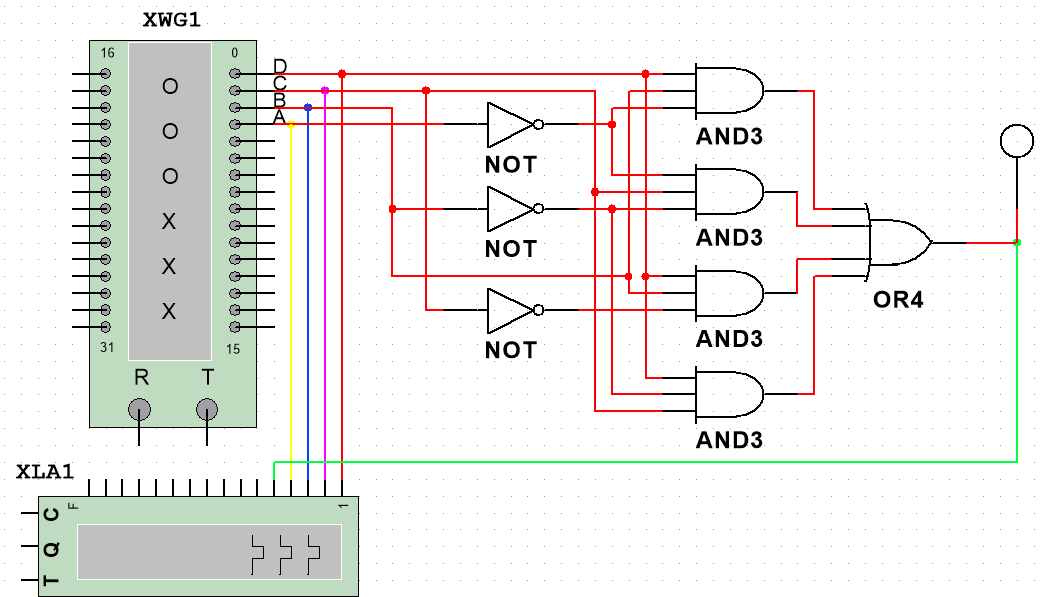
\includegraphics[width=\textwidth]{uklad_2.png}
    \caption{Układ logiczny w programie Multisim do ćwiczenia 2}
\end{figure}

\begin{figure}[H]
    \centering
    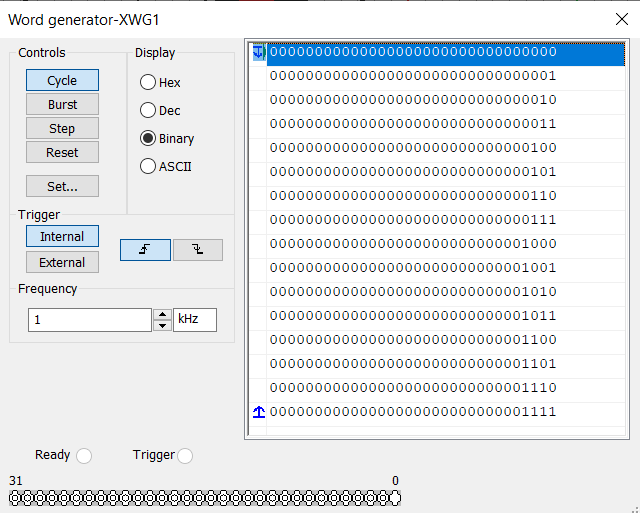
\includegraphics[width=\textwidth]{generator_2.png}
    \caption{Generator słów dla układu z ćwiczenia 2}
\end{figure}

Analogicznie jak w przypadku ćwiczenia pierwszego, przeprowadzona została analiza za pomocą analizarota logicznego. 
Jego wyniki zostały przedstawione \textbf{rysunku 15} (\textbf{A} - żółty, \textbf{B} - niebieski, \textbf{C} - różowy, 
\textbf{D} - czerwony, \textbf{wynik} - zielony). Układ dziala poprawnie.

\begin{figure}[H]
    \centering
    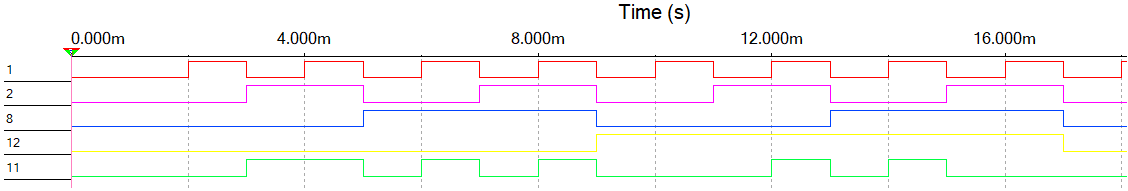
\includegraphics[width=\textwidth]{analiza_2.png}
    \caption{Wykres przebiegu czasowego badanego układu}
\end{figure}

\newpage
Poniżej alternatywny układ dla równania po przekształceniu
\[f(A,B,C,D)=\overline{B}C(\overline{A}+D)+BD(\overline{A}+\overline{C})\]

\begin{figure}[H]
    \centering
    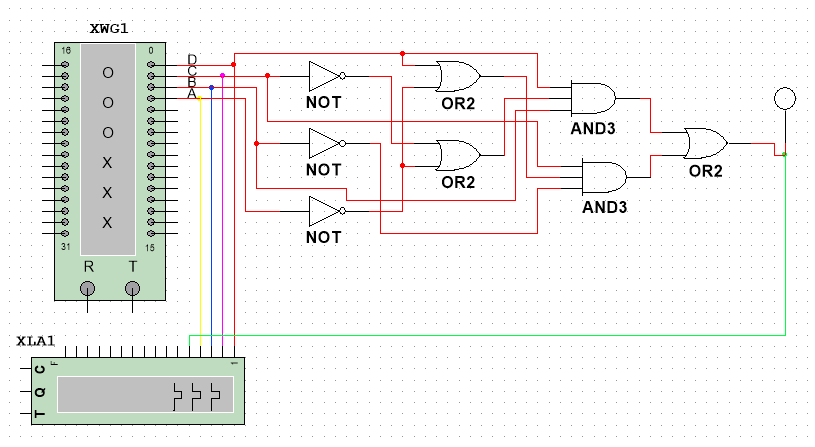
\includegraphics[width=\textwidth]{uklad_2_improved.png}
    \caption{Alternatywny układ do ćwiczenia 2}
\end{figure}

Oraz wykres jego analizatora (generator słów identyczny jak w przypadku pierwszej części układu)

\begin{figure}[H]
    \centering
    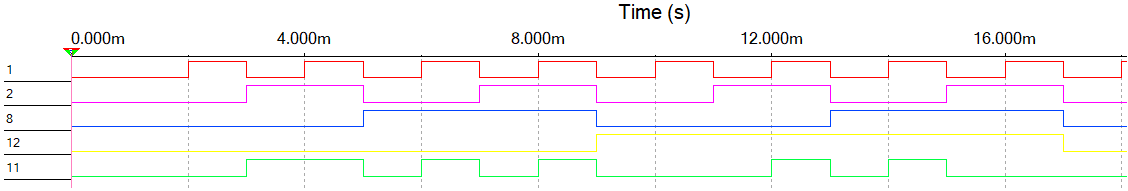
\includegraphics[width=\textwidth]{analiza_2.png}
    \caption{Wykres przebiegu czasowego alternatywnego układu}
\end{figure}

Poniżej (\textbf{na rysunku 18}) znajduję się automatyczny układ testujący sprawdzający poprawność działania układu

\begin{figure}[H]
    \centering
    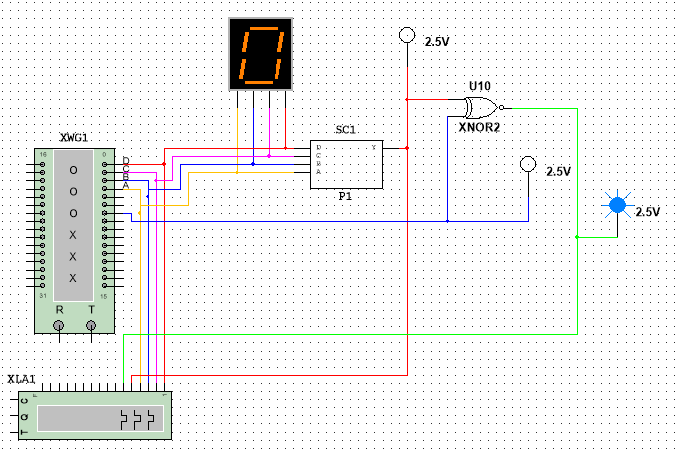
\includegraphics[width=\textwidth]{test_2.png}
    \caption{Automatyczny układ testujący dla układu 1b}
\end{figure}

\begin{figure}[H]
    \centering
    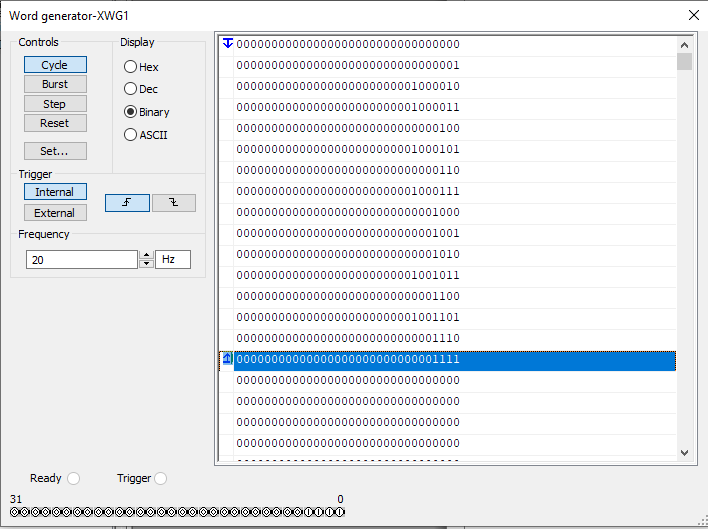
\includegraphics[width=\textwidth]{generator_test_2.png}
    \caption{Generator słów dla automatycznego układu testującego}
\end{figure}

\begin{figure}[H]
    \centering
    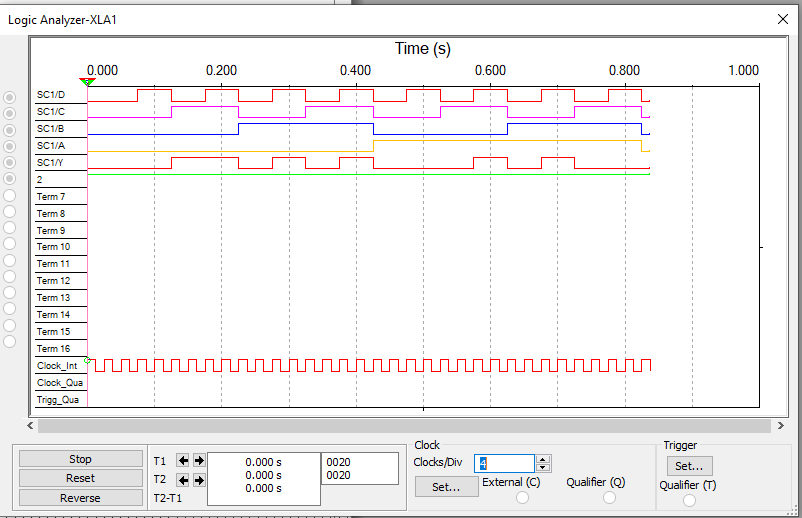
\includegraphics[width=\textwidth]{analiza_test_2.png}
    \caption{Analizator dla automatycznego układu testującego}
\end{figure}

\subsection{Wnioski}
\begin{itemize}
    \item
    W rzeczywistości ceny i dostępność różnych bramek różnią się, dlatego opłaca się, a nawet trzeba zmieniać 
    wejściowe funkcje logiczne na równoważne, by móc zastosować tańsze bramki.
    \item
    Metoda Karnough jest dobrym sposobem na generowanie minimalnej (lub bardzo uproszczonej) 
    funkcji logicznej, którą potem łatwiej wyrazić za pomocą układu cyfrowego.
    \item
    Układ może posłużyć do generowania liczb pierwszych używanych w algorytmie szyfrowania RSA.
\end{itemize}

\end{document}